\documentclass[xcolor={dvipsnames}]{beamer}
\usepackage{HECbeamer}
\uselanguage{French}
\languagepath{French}
\title[\color{white}{MATH60604 \S~2g - Interactions}]{MATH60604 \\Modélisation statistique \\ \S~2g - Interactions}
\author{}
\date{\today}
\institute{HEC Montréal\\
Département de sciences de la décision}
\date{} 

\begin{document}
\frame{\titlepage}
\begin{frame}
 \frametitle{Interactions}
 \bi 
 \item On parle d'\textbf{interaction} lorsque des combinaisons de variables explicatives affectent la variable réponse différemment que lorsqu'elles sont considérées individuellement.
 \item par ex., les primes d'assurance santé sont différentes pour les fumeurs en fonction de leur surpoids: les obèses paient une surprime.
\item On dit que les variables $\mathrm{X}_1$ et $\mathrm{X}_2$ interagissent sur $Y$ quand \alert{l'effet de $\mathrm{X}_1$ sur $Y$ dépend de la valeur de $\mathrm{X}_2$, et vice-versa}.
  \item On considère les données fictives \code{interaction} pour illustrer cette notion.
  \ei
 \end{frame}
 
\begin{frame}[fragile]
\frametitle{Interaction entre une variable continue et une variable binaire}
\bi
\item On utilise seulement deux variables, le \code{sexe} et le temps de \code{fixation}, pour modéliser l'\code{intention} d'achat. 
\item Le modèle sans interaction est
\begin{align*}
\code{intention}=\beta_0 + \beta_1 \code{sexe} + \beta_2 \code{fixation} + \varepsilon,
\end{align*}
où \code{sexe} est une variable binaire égale à \code{1} pour les femmes et \code{0} pour les hommes.
\ei
\begin{tcolorbox}[colback=white,colframe=hecblue,title=code \SASlang pour ajuster un modèle linéaire]
\begin{verbatim}
proc glm data=infe.interaction;
class sexe(ref="0");
model intention=sexe fixation / ss3 solution;
run;
\end{verbatim}
\end{tcolorbox}
\end{frame}


 \begin{frame}[fragile]
\frametitle{Absence d'interaction }
\bi
\item Le modèle n'inclut pas d'interaction entre \code{fixation} et \code{sexe}.
\item Dans le modèle postulé, l'effet de la variable continue \code{fixation} est \alert{identique} pour les deux modalités de la variable binaire. 
\item Inversement, l'effet de la variable binaire est la même pour toutes les valeurs de la variable continue. Le graphique montrerait ainsi que la pente est la même peut importe le \code{sexe} et que les droites de régression sont \alert{parallèles}. 
\ei
\begin{figure}
 \centering
 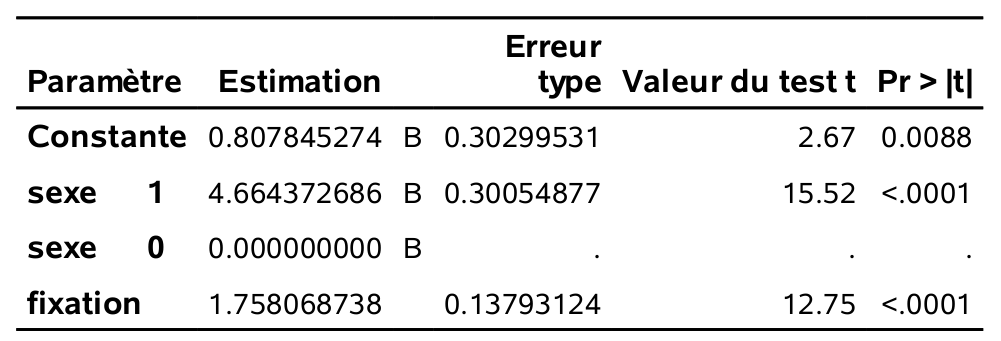
\includegraphics[width=0.65\linewidth]{img/c2/diapos3-e18}
\end{figure}
{ \footnotesize Tous les paramètres sont significatifs à niveau $\alpha =0.05$.}
\end{frame}

 \begin{frame}[fragile]
  \frametitle{Illustration d'une interaction binaire-continue}
  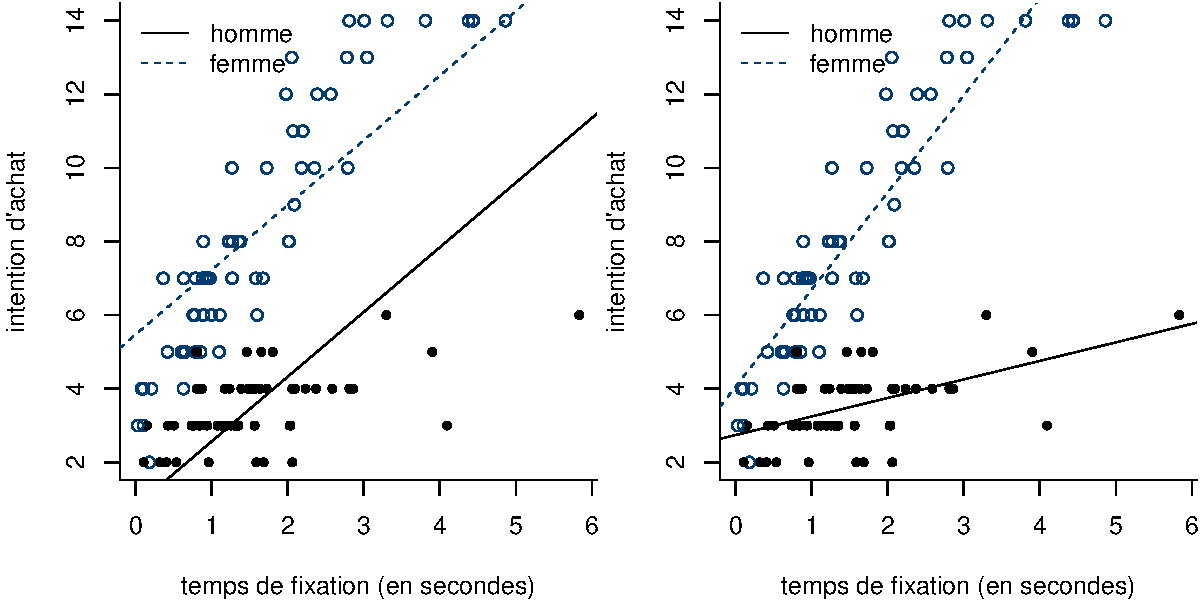
\includegraphics[width =\textwidth]{img/c2/03-linreg-interaction_cont_fr.pdf}
 \end{frame}


\begin{frame}[fragile]
\frametitle{Modéliser l'interaction}
\bi 
\item La figure de droite montre qu'un meilleur modèle incluerait des \alert{\textbf{pentes différentes}} pour les hommes et les femmes.
\item  Pour ce faire, il suffit de  \alert{créer une nouvelle variable égale au produit} \code{fixation} $\cdot$ \code{sexe} et de l'ajouter au modèle,
{\small 
\begin{align*}
\code{intention} = \beta_0 + \beta_1 \code{sexe} + \beta_2\code{fixation} + \beta_3 \code{fixation}\cdot \code{sexe} + \varepsilon.
\end{align*} 
}
\item Selon le niveau de la variable \code{sexe}, on a
{\small 
\begin{align*}
\code{intention} = 
\begin{cases}
(\beta_0 + \beta_1) + (\beta_2 + \beta_3)\code{fixation} + \varepsilon, & \text{ si } \code{sexe}=1,\\
  \beta_0 + \beta_2 \code{fixation} + \varepsilon, & \text{ si } \code{sexe}=0.                  
\end{cases}
\end{align*} 
}
\item On recouvre le modèle avec  \alert{effets principaux}  quand $\beta_3$ est nul. 
\ei
\end{frame}

 \begin{frame}[fragile]
\frametitle{Interaction entre variables continue et binaire}
% \bi
% \item Here is the \SASlang code to fit the model with interaction
% \ei
\begin{tcolorbox}[colback=white,colframe=hecblue,title=Code \SASlang pour ajuster le modèle linéaire avec une interaction]
{\small 
\begin{verbatim}
proc glm data=infe.interaction;
class sexe(ref="0");
model intention=sexe fixation fixation*sexe 
    / ss3 solution;
run;
\end{verbatim}
}
\end{tcolorbox}
\end{frame}
\begin{frame}
\frametitle{Estimés des coefficients du modèle avec interaction}
\begin{center}
  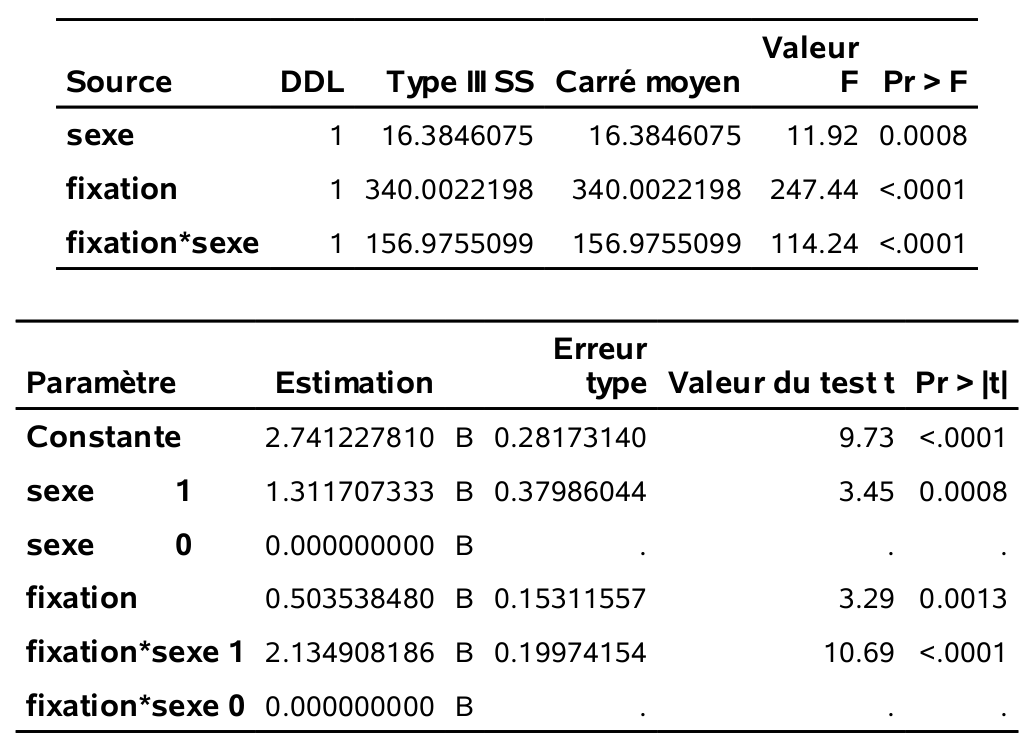
\includegraphics[width = 0.8\linewidth]{img/c2/diapos3-e19}
\end{center}

\end{frame}

\begin{frame}
\frametitle{Interaction entre variables continue et binaire}
\bi
% \item If we want to test whether the slopes are different, that is, if the effect of
% \code{fixation} is different according to the value of \code{sexe}, \alert{we only need to test whether the parameter $\beta_3$ is significantly different from 0}. 
\item Tester si l'interaction est significative revient à tester $\Hy_0: \beta_3=0$.
\item Si on rejette $\Hy_0$, il y a une interaction significative entre les deux variables (dans l'exemple, la valeur-$p$ est plus petite que $0.0001$). 
\item Le modèle ajusté avec l'interaction est
\bi
\item quand \code{sexe}$=\code{0}$, on obtient $\E{\code{intention}}=2.74+0.50  \code{fixation}$;
\item quand \code{sexe}$=\code{1}$, on obtient $\E{\code{intention}}=4.05+2.64  \code{fixation}$.
\ei
\item Le concept d'interaction peut être directement généralisé au cas d'une interaction entre variable continue et variable catégorielle à $k$ niveaux.
\bi    
\item Dans ce cas, on doit regarder le test $F$ afin de vérifier si l'interaction est significative.
\ei
 \ei
\end{frame}


% \item Once again, as we've seen for powers of a variable, it's possible to directly model the product of two variables using the command \code{model} for \code{proc glm}. 
% \bi
% \item \SASlang will consider \code{fixation}$*$\code{sexe} as interaction term between the two covariates.
% \ei


 \begin{frame}
\frametitle{Note technique}
\bi
\item Les tests pour \code{fixation} ne sont pas les mêmes dans les deux tableaux, parce que  \code{fixation} est inclus dans une interaction avec une variable catégorielle \code{class}.
\item Dans le tableau des coefficients, la valeur-$p$ teste l'hypothèse bilatérale $\Hy_0:\beta_2=0$, correspondant à l'effet de \code{fixation}
quand \code{sexe=0}.
\item Dans le tableau au dessus, le test est pour l'effet moyen de \code{fixation}, à savoir
\begin{align*}
\Hy_0: \{\beta_2+(\beta_2+\beta_3)\}/2=0
\end{align*}
\item Ces tests sont \textbf{sans} intérêt. On ne peut retirer l'effet principal $\beta_2$ tant que l'interaction est présente.
\ei
\end{frame}
 \begin{frame}
  \frametitle{Paramétrisation arbitraire et effets principaux}
  \bi \item Dans le modèle d'\code{intention} en fonction du \code{sexe} et du temps de \code{fixation},  on ne retirerait pas l'effet principale \code{fixation} en conservant \code{fixation*sexe} même si l'effet de fixation n'est pas significatif.
  \item Cela s'explique par le fait que $\beta_2$ est la pente pour les hommes. Sans \code{fixation}, le modèle devient 
\begin{align*}
\code{intention} = 
\begin{cases}
(\beta_0 + \beta_1) + \beta_3\code{fixation} + \varepsilon, & \text{ si } \code{sexe}=1,\\
  \beta_0 + \varepsilon, & \text{ si } \code{sexe}=0;                 
\end{cases}
\end{align*}  
cela impliquerait que l'intention d'achat est constante pour les hommes, peu importe le temps de fixation.
\item Puisque la catégorie de référence est arbitraire, en changeant la paramétrisation de \code{sexe} (\code{0} pour les femmes, \code{1} pour les hommes), on changerait le modèle et donc l'inférence.
\item Le niveau de référence de la variable catégorielle ne serait donc plus arbitraire.
\ei
 \end{frame}

\begin{frame}
\frametitle{Interactions entre variables catégorielles - théorie}
\bi
\item Pour deux variables catégorielles avec  $k_1$ et $k_2$ niveaux, le modèle d'interaction a \[k_1k_2 = 1+ (k_1-1) + (k_2-1) + (k_1-1)(k_2-1)\] paramètres --- un par combinaison.
\item Le nombre de paramètres additionnels par rapport au modèle avec effets principaux est $(k_1-1)(k_2-1)$.
\item L'interprétation des effets principaux est comme à l'accoutumée, soit un contraste relativement à un niveau de base. Ce dernier change selon que l'on inclue (ou pas) l'interaction.
\item On considère une interaction \textbf{seulement si} l'effet principal correspondant est déjà inclus dans le modèle.
\item Si la variance des sous-groupes est égale, on peut tester l'interaction en utilisant une statistique $F$.
\ei
\end{frame}
\begin{frame}[fragile]
 \frametitle{Interactions entre variables catégorielles}
 \bi 
 \item Considérez un modèle pour les primes d'assurance en fonction du facteur obésité et du statut de fumeur. On filtre préalablement l'effet de l'âge.
 \item Le modèle avec effets principaux pour chaque groupe est
\begin{align*}
\code{rcharges} = \beta_0 + \beta_1 \code{fumeur} + \beta_2 \code{obese}_1 +  \beta_3 \code{obese}_2 + \eps. 
\end{align*}
où $\code{obese}_1=1$ si $25\leq \code{imc} < 30$ (surpoids) et $\code{obese}_2=1$ si $\code{imc} \geq 30$ (obèse).
\ei

\end{frame}
\begin{frame}[fragile]
 \frametitle{Représentation graphique de l'interaction entre variables catégorielles}
\begin{figure}
 \centering
 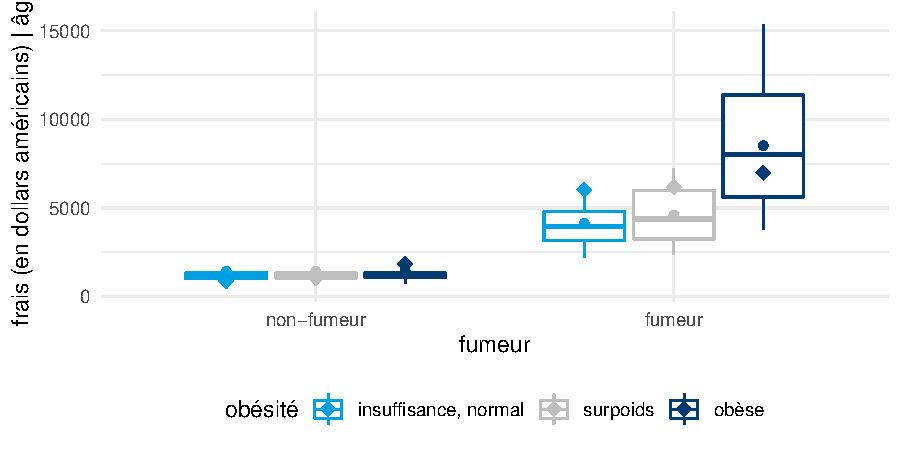
\includegraphics[width = 0.8\linewidth]{img/c2/03-linreg-interaction_categ_fr.pdf}
\end{figure} 
{\tiny 
Les losanges indiquent la valeur ajustée (moyenne) de chaque groupe pour le modèle sans interaction et les cercles celles du modèle avec interaction. Les primes sont clairement plus élevées pour les fumeurs obèse, une réalité que le modèle avec effets principaux n'arrivent pas à capturer : il sous-estime les frais pour les fumeurs obèses et surestime ceux des fumeurs non-obèses.  \par
}
\end{frame}
\begin{frame}[fragile]
\frametitle{Modèle avec interaction entre deux variables catégorielles}
Le modèle linéaire avec l'interaction est
{ \small 
\begin{align*}
\code{rcharges} &= \beta_0 + \beta_1 \code{fumeur} + \beta_2 \code{obese}_1 +  \beta_3 \code{obese}_2 + \\ & \quad \beta_4\code{fumeur}\cdot\code{obese}_1  + \beta_5\code{fumeur}\cdot\code{obese}_2  + \eps. 
\end{align*}
}
La moyenne des frais (une fois l'impact de l'âge pris en compte) est
{\small 
\bi 
\item $\beta_0$ pour les non-fumeurs dont l'indice de masse corporelle est inférieur à 25;
\item $\beta_0 + \beta_2$ pour les non-fumeurs en surpoids;
\item $\beta_0 + \beta_3$ pour les non-fumeurs obèses;
\item $\beta_0 +\beta_1+  \beta_3 + \beta_5$ pour les fumeurs obèses\ldots 
\ei
}
Tester si l'interaction est significative revient à tester $\Hy_0: \beta_4=\beta_5=0$.
\end{frame}
\begin{frame}[fragile]
\frametitle{Interprétation des paramètres du modèle avec interaction}
Le modèle linéaire avec l'interaction est
{ \small
\begin{align*}
\log(\code{charges}) &= \beta_0 + \beta_1 \code{fumeur} + \beta_2 \code{obese}_1 +  \beta_3 \code{obese}_2+ \\ & \quad \beta_4\code{fumeur}\cdot\code{obese}_1  + \beta_5\code{fumeur}\cdot\code{obese}_2  + \eps. 
\end{align*}
}\vspace{-0.5cm}
 \bi
  \item L'interprétation est comme d'habitude, mais l'effet des paramètres individuels est parfois difficile à isoler.
{\small 
\bi
\item $\beta_0$, représente la moyenne des frais des individus non-fumeurs dont l'IMC est inférieur à 25.
\item $\beta_1$ est la surprime par rapport à la catégorie de base pour les fumeurs dont l'IMC est inférieur à 25.
\item $\beta_2$ est la surprime  pour les gens en surpoids par rapport à la catégorie de base (tous non-fumeurs).
\item $\beta_3$  est la surprime  pour les obèses non-fumeurs par rapport aux gens dont l'IMC est inférieur à 25 (tous non-fumeurs).
\item $\beta_1+\beta_4$  est la surprime pour les fumeurs en surpoids (relativement aux non-fumeurs en surpoids).
\item $\beta_3 + \beta_5$  est la surprime des fumeurs obèses par rapport aux fumeurs dont l'IMC est inférieur à 25.
\ei
}
\ei
\end{frame}




\begin{frame}
 
\frametitle{Interaction d'ordre supérieur}
\bi
% \item Tous les exemples précédents étaient des illustrations d'interactions d'ordre deux, c'est-à-dire, entre deux variables. 
\item En théorie, on peut avoir une interaction entre un nombre quelconque de variables. En pratique, on dépasse rarement l'ordre trois car il devient rapidement difficile d'interpréter correctement les effets et estimer une interaction entre plusieurs variables demande une grande taille d'échantillon. 
\item Le principe de base est toujours le même. Pour créer une interaction d'un ordre donné entre des variables, il faut que tous les termes d'interactions d'ordre inférieur entre ces variables soient également présents. 
\item On interprète l'effet des variables en fixant les valeurs des autres avec qui elles interagissent. 

\ei
\end{frame}


\begin{frame}[fragile]
\frametitle{Remarques sur les interactions}
\bi
\item Il faut toujours inclure les termes d'ordre inférieurs, même si ils ne sont pas significatifs, puisqu'ils sont nécessaires pour l'inférence.
\item Il est tentant d'inclure plusieurs interactions entre des variables catégorielles, mais faites attention aux sous-catégories où il y a peu d'observations.
\item Les algorithmes qui servent à la sélection de modèles basent leur choix sur des critères de performance prédictive et à ce titre enlèvent parfois les termes principaux tout en gardant les interactions.
\bi \item Cela n'a peut être pas d'importance pour la construction d'une boîte-noire.
\ei
\item En enlevant les effets principaux, la catégorie de base n'est \textbf{plus arbitraire} et l'inférence est \textbf{invalide}.

% \item One exception is when we're developing a predictive model and we don't plan on testing individual variables.  We would then include all the variables, as well as several (or even all) interaction terms and let an algorithm choose the best model. 
% \item This algorithm will not necessarily respect the above rule, but this won't matter as we only care about predictive performance.
\ei
\end{frame}
\end{document}
